% +---------------------------------------------------------------+
% | Author :    Noémie Plancherel, HEIG-VD
% | Date :      04.10.2022
% +---------------------------------------------------------------+

\chapter{Analyse de menaces}
\label{ch:analyse_menaces}

Ce chapitre a pour but d'identifier et analyser toutes les menaces existantes et / ou potentielles des \textit{password managers} en les modélisant en suivant un certain processus afin d'avoir une meilleure vision des risques.

Puis, nous allons rédiger toutes les exigences sécuritaires que doivent respecter les gestionnaires de mots de passe afin que ces dernières garantissent une utilisation sûre qui évite des pertes, un vol de données, une usurpation d'identité, des accès aux services, etc.

\section{Modélisation de menaces}
Afin de modéliser correctement les menaces, nous allons suivre la norme ISO 27005\cite{ISO27005}. Cela va nous permettre de séparer la modélisation en un processus avec plusieurs étapes comme suit:

\begin{enumerate}
	\item Établissement du contexte, qui inclut
	\begin{itemize}
		\item Objectifs des gestionnaires de mots de passe
		\item Hypothèses et exigences de sécurité
		\item Actifs à haute valeur 
		\item Data Flow Diagram
		\item Définition des critères d'analyse
	\end{itemize}
	\item Identification des risques
		\begin{itemize}
		\item Identification des biens
		\item Identification des menaces
		\item Identification des contrôles
		\item Identification des vulnérabilités
		\item Identification des conséquences
	\end{itemize}
	\item Analyse des risques
	\item Évaluation des risques
	\item Traitement des risques
	\item Documentation 
\end{enumerate}
La dernière étape ne sera pas explicitement abordée car elle vise à documenter le modèle de menaces que nous allons établir.

Pour chaque étape du processus, nous allons aborder les 3 types de gestionnaires que nous avons cité précédemment: local-based, browser-based et cloud/local-based. Étant donné que les applications browser-based et cloud/local-based fonctionnent les deux en local et en cloud avec la synchronisation de données, nous pouvons nous baser sur deux catégories uniquement; les gestionnaires \textbf{local-based} et \textbf{cloud/local-based}. 

Nous allons également nous baser sur le processus de modélisation de menaces de OWASP\cite{owasp}.

Il est intéressant de mélanger les deux méthodologies car la norme ISO est plus axée sur une gestion des risques alors que OWASP se base sur une modélisation des menaces. Les deux ont des points communs notamment au niveau de la description et la décomposition de l'application, néanmoins la norme ISO va plus en profondeur en identifiant tous les risques possibles (vulnérabilités, menaces, conséquences, etc.). OWASP a également ses avantages en schématisant le flux de données à l'aide de DFDs (\textit{Data Flow Diagram}) et en catégorisant les menaces avec le modèle STRIDE. \newpage

\subsection{Définition des critères}

Avant de commencer, nous allons définir les différents critères et niveaux pour évaluer l'impact des événements (les conséquences), la probabilité d'événement, la sévérité des vulnérabilités ainsi que l'évaluation des risques. Ces niveaux seront réutilisés pour l'identification des risques dans la suite de l'analyse de menaces.

\begin{table}[H]
	\begin{tabular}{llc}
		\hline
		Échelle  & Description                                                                                                                                                                                               & Valeur   \\ \hline
		Aucune   & La vulnérabilité ne présente aucune sévérité                                                                                                                                                              & 0        \\
		Bas      & \begin{tabular}[c]{@{}l@{}}La vulnérabilité a peu d'impact sur l'entreprise et demande un\\ accès physique ou local au système\end{tabular}                                                               & 0.1-39   \\
		Moyen    & \begin{tabular}[c]{@{}l@{}}En général, elle demande à l'attaquant d'être sur le même réseau \\ que la victime et elle demande les privilèges utilisateurs pour \\ effectuer une exploitation\end{tabular} & 4.0-6.9  \\
		Haut     & \begin{tabular}[c]{@{}l@{}}La vulnérabilité est difficile à exploter, peut être une élévation de \\ privilèges et peut amener à une importante perte de données ou \\ de temps d'arrêt\end{tabular}       & 7.0-8.9  \\
		Critique & \begin{tabular}[c]{@{}l@{}}Exploitation de vulnérabilités au niveau root, l'attaquant n'a pas\\ besoin d'être authentifié ou avoir des connaissances sur la victime\end{tabular}                          & 9.0-10.0 \\ \hline
	\end{tabular}
	\caption{Scores de sévérité basés sur CVSS v3.1}
\end{table}

\begin{table}[H]
	\centering
	\resizebox{\textwidth}{!}{\begin{tabular}{llc}
			\hline
			Échelle        & Description                                                                                                                                                                                                    & Valeur \\ \hline
			Négligeable    & L'impact sur l'entreprise est négligeable                                                                                                                                                                      & 0      \\
			Mineur         & \begin{tabular}[c]{@{}l@{}}L'effet sur les biens de l'entreprise est limité, comme entraîner des \\ pertes financières mineures ou entraîner des dommages mineures \\ aux actifs de l'entreprises\end{tabular} & 1      \\
			Modéré         & \begin{tabular}[c]{@{}l@{}}L'effet sur les biens peut être grave, les effets causés sur les biens \\ seront considérés comme importants\end{tabular}                                                           & 2      \\
			Important      & L'effet sur les biens de l'entreprise peut être grave à catastrophique                                                                                                                                         & 3      \\
			Catastrophique & \begin{tabular}[c]{@{}l@{}}On s'attend à ce que la menace ait de multiples effets graves à \\ catastrophiques sur les biens de l'entreprise\end{tabular}                                                       & 4      \\ \hline
	\end{tabular}}
	\caption{Impact des menaces sur l'entreprise}
\end{table}

\begin{table}[H]
	\centering
	\begin{tabular}{llc}
		\hline
		Échelle      & Description                                            & Valeur \\ \hline
		Rare         & La probabilité que l'événement arrive est rare         & 0      \\
		Peu probable & La probabilité que l'événement arrive est peu probable & 1      \\
		Possible     & La probabilité que l'événement arrive est possible     & 2      \\
		Probable     & La probabilité que l'événement arrive est probable     & 3      \\
		Certain      & La probabilité que l'événement arrive est certain      & 4      \\ \hline
	\end{tabular}
	\caption{Probabilités d'événements}
\end{table}

Pour l'évaluation des risques, il est important de prendre en considération la probabilité d'événements et les conséquences sur l'entreprise afin de définir une échelle d'évaluation de risques. Nous utilisons une matrice de risques basée sur une étude quantitative\cite{matrix}.

\begin{figure}[H]
	\centering
	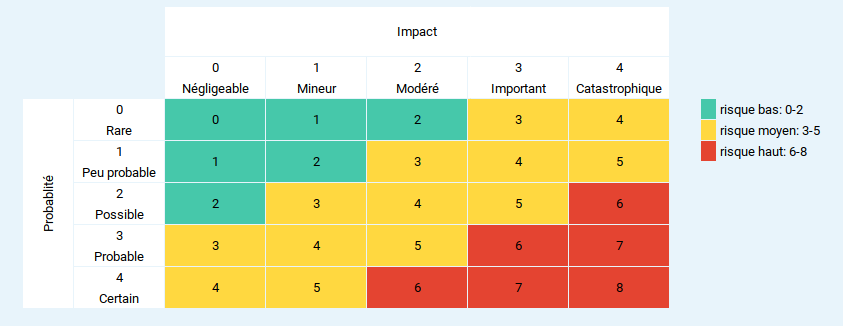
\includegraphics[width=15.5cm]{images/risque_evaluation.png}
	\centering
	\caption{Critères d'évaluation des risques \label{Critères d'évaluation des risques}}
\end{figure}

\subsection{Établissement du contexte}
Dans cette section, nous allons comprendre les applications et comment interagissent les gestionnaires de mots de passe avec les entités externes. Au final, nous allons établir un \textit{Data Flow Diagram} (DFD) qui va nous permettre de présenter tous les chemins différents du système en mettant en avant les vulnérabilités potentielles.

\textbf{Objectifs du système}

Comme cité plusieurs fois, l'objectif principal d'un gestionnaire de mots de passe est de stocker de manière \textbf{sûre} des informations sensibles, le plus souvent des identifiants, mais également la possibilité de stocker des notes, des informations bancaires, contrats, etc. Ils offrent également la fonctionnalité de générer des mots de passe forts et d'auto-compléter les champs de connexion. 

Tout dépend, du gestionnaire de mots de passe, ils peuvent offrir une fonctionnalité de backup, afin de sauvegarder le coffre-fort et de garantir une perte minimale de données au cas où. Il existe également la fonctionnalité de partage de données entre utilisateurs.

Pour les applications qui fonctionnent avec le cloud et qui ne sont pas 100\% offline, l'utilisateur a la possibilité de synchroniser ses données entre appareils (desktop, mobile, navigateur, smartwatch). 

\textbf{Hypothèses de sécurité}

On peut émettre plusieurs hypothèses de sécurité afin de mettre en avant ce que doit assurer le gestionnaire de mots de passe pour être considéré comme sûr. Nous allons lister les hypothèses afin que cela soit le plus clair possible :

\begin{itemize}
	\item Données du gestionnaire soient chiffrées et protégées en RAM, sur le disque ainsi que lors de communications avec les serveurs. Nous définissons les données comme étant le coffre-fort, avec tous les identifiants, les clés et le master password. 
	\item Serveurs de confiance
\end{itemize}

Ceux-ci étant les plus importants afin de garantir la meilleure sécurité possible sur l'application, nous irons plus en détails dans la section sur les exigences sécuritaires.

\textbf{Actifs de valeurs}

Nous pouvons à présent définir les actifs (\textit{assets}) des gestionnaires de mots de passe, qui représentent les éléments qui ont de la valeur et qui demandent une importante protection. 

Tout d'abord, un actif à haute valeur est le \textbf{gestionnaire de mot passe} qui représente l'application. Cette dernière peut être sous forme d'application desktop, extension de navigateur ou application mobile. Un utilisateur ou un administrateur devrait pouvoir se connecter à l'application pour avoir accès à son coffre-fort.

Ensuite, un autre bien important est \textbf{le coffre-fort} qui contient tous les identifiants, notes, informations bancaires, etc. stockées par l'utilisateur, qui peut être représenté comme une base de données. Le bien principal sont donc les données, qui sont chiffrées et protégées. Un utilisateur devrait ainsi avoir l'habilité d'avoir accès à son coffre-fort en clair et de pouvoir y ajouter au minimum des identifiants.

Un actif qu'on peut également ajouter est le \textbf{master password} entré l'utilisateur pour déverrouiller le gestionnaire de mots de passe et avoir accès à son coffre-fort. Cet élément est très important car il va permettre de dériver les clés de chiffrement et ainsi, de pouvoir avoir accès au coffre-fort en clair.

Un autre actif à haute valeur sont les \textbf{clés}. Nous incluons dans cet actif les clés de chiffrement ainsi que les clés privées lors du partage de données entre utilisateurs. Nous pouvons ajouter le processus de génération de clés.

Dans le cadre de gestionnaires de mots de passe cloud/local-based qui ne fonctionnent pas en mode offline, nous voulons protéger les données des \textbf{serveurs du constructeur}. Le processus de transfert de données, c'est-à-dire la communication, est également important car les données doivent impérativement être protégées. Nous pouvons inclure les fonctionnalités de synchronisation de données et le partage de données entre utilisateur, qui demandent de passer par les serveurs du constructeur.

Un asset important à ajouter sont les \textbf{données partagées} entre utilisateurs lors de la fonctionnalité de partage. La ou les données échangées doivent être sécurisées afin de ne pas les exposer à n'importe quel utilisateur. 

Finalement, nous pouvons ajouter comme dernier actif, les fichier de \textbf{backups} qui devraient être chiffrés et protégés sur les devices de l'utilisateur ou des serveurs du provider.

À présent, pour effectuer une analyse de menaces la plus claire et structurée possible, nous allons séparer l'application en plusieurs parties comme suit:

\begin{enumerate}
	\item[\textbf{M1}] Coffre-fort standalone, local-based (haut-niveau)
	\item[\textbf{M2}] Fonctionnalité de backup
	\item[\textbf{M3}] Fonctionnalité de synchronisation (pour les gestionnaires cloud-based)
	\item[\textbf{M4}] Fonctionnalité de partage
	\item[\textbf{M5}] Sécurité de l'application et ses composants (bas-niveau)
\end{enumerate}

Pour chaque étape, nous identifierons et analyserons les risques pour couvrir tous les aspects et les fonctionnalités d'un gestionnaire de mots de passe. UN code d'identification a été ajouté afin de mieux organiser l'analyse.

Nous ferons un récapitulatif à la fin en évaluant tous les risques définis sur toutes les étapes et en listant toutes les contre-mesures nécessaires à prendre.
\newpage

\subsection{M1 Application haut-niveau}

La première partie qu'on analyse, définit une application standalone toute simple, qui est un gestionnaire de mots de passe qui ne fonctionne qu'en local et qui interagit avec aucune entité externe. Premièrement, nous avons effectué un DFD (\textit{Data Flow Diagram}) afin de constater les processus principaux de l'application :

\begin{figure}[H]
	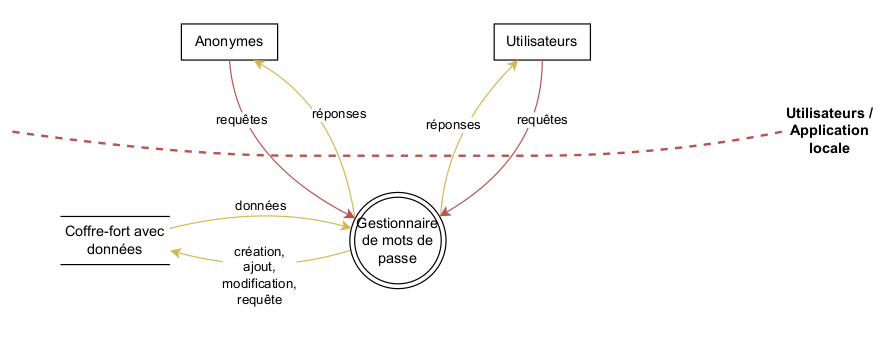
\includegraphics[width=13cm]{images/dfd_local.png}
	\centering
	\caption{Data Flow Diagram pour les gestionnaires M1}
\end{figure}

\subsubsection{Identification des risques}
Cette section va nous servir à déterminer ce qui peut se produire pour causer un dommage et à comprendre comment, où et pourquoi l'incident peut se produire. 

Afin d'établir une étude complète, nous allons premièrement identifier les biens, menaces (avec les sources de menaces et les scénarios), les contrôles, les vulnérabilités ainsi que les conséquences sur l'entreprise.

\textbf{Identification des biens}

Nous avons déjà identifié les actifs plus-haut dans l'analyse, cependant nous allons identifier les actifs présents dans une application standalone. De plus, nous allons ajouter un code pour les identifier et les référencer plus tard dans l'identification des risques.

\begin{table}[H]
	\centering
	\resizebox{\textwidth}{!}{\begin{tabular}{lll}
		\hline
		Code & Bien                                & Description                                                           \\ \hline
		A1   & Gestionnaire de mots de passe & L'application du gestionnaire de mots de passe                      \\
		A2   & Coffre-fort                     & Base de données avec toutes les informations stockées                \\
	    A3  & Master password                   & Mot de passe principal afin de déchiffrer le coffre-fort               \\
		\hline
	\end{tabular}}
\caption{Biens des gestionnaires de mots de passe M1}
\end{table}
\textbf{Identification des sources de menaces}

Nous allons identifier toutes les sources de menaces possibles des gestionnaires de mots de passe avec leurs motivations (uniquement si c'est de source humaine) afin de pouvoir mettre en avant les différents scénarios de menaces.

\begin{table}[H]
	\centering
	\begin{tabular}{cll}
		\hline
		Code & Source de menace                & Motivations                               \\ \hline
		S1   & Hackers & Amusement, gloire, challenge, argent, ego \\
		S2   & Script kiddies                  & Curiosité, ego, argent, amusement         \\
		S3   & Concurrent                      & Espionnage, réutilisation de contenu      \\
		S4   & Cybercrime                      & Argent, destruction de données            \\
		S5   & Accident humain                 & -                                         \\
		S6   & Problèmes techniques            & -                                         \\ \hline
	\end{tabular}
\caption{Sources de menaces des gestionnaires de mots de passe M1}
\end{table}

Ci-dessous, se trouve un tableau avec différents scénarios d'attaques par rapport aux biens que nous avons défini précédemment. Nous nous basons sur le modèle STRIDE\footnote{\href{https://owasp.org/www-community/Threat_Modeling_Process}{https://owasp.org/www-community/Threat\_Modeling\_Process}} afin de définir les types de menaces. 
\begin{table}[H]
		\centering
	\resizebox{\textwidth}{!}{\begin{tabular}{ccclll}
			\hline
			& Code & Code du bien & Scénario de menace                                                                                                            & Type de menace                & Source de menace    \\ \hline
			2 & T2   & A1, A3           & \begin{tabular}[c]{@{}l@{}}Key-logger installé sur le device de l'utilisateur \\ et qui sniff le master password\end{tabular} & \textit{Elevation of privileges}    & S1, S2, S4        \\
			2 & T2   & A1           & \begin{tabular}[c]{@{}l@{}}Utilisateur non-déconnecté de son compte \\et attaquant a accès au device\end{tabular}                                                                                     & \textit{Elevation of privileges}      & S1, S2, S4, S5   \\
			3 & T1   & A1           & Mauvais mécanisme d'authentification                                                                                          & \textit{Spoofing}    & S1, S2, S4, S6    \\
			4 &T3   & A1           & Lecture du presse-papier                                                                                                      & \textit{Information disclosure}    & S1, S2, S4       \\                                                                                
			5 & T1   & A1           & \begin{tabular}[c]{@{}l@{}}Coffre-fort compromis dû à des identifiants volés\\ sur d'autres sites\end{tabular}                & \textit{Spoofing}      & S1, S2, S4, S5   \\
			6 & T3   & A2           & \begin{tabular}[c]{@{}l@{}}Récupération du coffre-fort et déchiffrement\\ dû à un algorithme trop simple\end{tabular}  & \textit{Information disclosure}    & S1, S2, S4      \\
			7 & T6   & A2           & Injection SQL dans la base de données utilisateur                                                                                                                           & \textit{Tampering}           & S1, S2, S4 	 \\  
			8 & T1   & A3           & Brute-force sur le master password                                                                                            & \textit{Spoofing}      & S1, S2, S4, S5  \\			
			9 & T1   & A3           & Phishing par mail pour récupérer le master password  	  & \textit{Spoofing}   & S1, S2, S3, S4    \\		                                                                                                         
			\\\\	\hline 
			\multicolumn{6}{l}{A1 = Gestionnaire de mots de passe | A2 = Coffre-fort | A3 = Master password}\\ \hline
	\end{tabular}}
\caption{Scénarios et types d'attaques possibles sur applications M1}
\end{table}

\textbf{Identification des contrôles}

Une étape importante lors de l'identification des risques est d'identifier les contrôles qui existent déjà sur les applications sur lesquelles nous basons notre analyse de risques. Étant donné, que notre étude est plutôt générale car elle ne se base pas sur un seul gestionnaire de mots de passe, nous allons énumérer les contrôles qui ont été entrepris afin de baisser le niveau de risque. Nous parlerons en détails des contrôles effectués lors de la seconde partie du travail.

Étant donné que dans cette partie, nous nous concentrons sur une application basique qui ne fonctionne qu'en local et que nous abordons pas le bas-niveau, nous n'irons pas en détails au niveau des contrôles. 

Ce qui existe déjà pour éviter des attaques sur mots de passe sont des critères qui sont, pour la plupart des gestionnaires, imposés par le constructeur. Ces critères exigent par exemple d'avoir un certain nombre de caractères afin d'avoir un master password fort.

Au niveau de la protection du keylogger, aucune protection n'est réellement implémentée, à part utiliser l'application dans environnement sécurisé comme \textit{Secure Desktop} sur Windows. Pour la protection du presse-papier, certaines applications (comme Keepass) mettent à disposition une fonctionnalité pour enlever les données sensibles du presse-papier et de la mémoire après un certain moment.

Pour le coffre-fort, la plupart des gestionnaires de mots de passe proposent un chiffrement fort du coffre-fort afin de protéger au mieux les données, afin que même si ce dernier est volé, la personne malveillante ne puisse pas le déchiffrer et récupérer les données stockées.

\textbf{Identification des vulnérabilités}

Pour chaque actif identifié au préalable, nous allons analyser les vulnérabilités qui pourraient être présentes. Nous allons également ajouter la sévérité de la vulnérabilité. 

\begin{table}[H]
	\centering
		\resizebox{\textwidth}{!}{\begin{tabular}{cll}
				\hline
				Bien                   & Vulnérabilité                                                                                                          & Sévérité de la vulnérabilité   \\ \hline
				A1                     & Temps de session long                                                                                                  & Critique                     \\
				A1                     & Presse-papier non nettoyé après un certain temps                                                                       & Moyen                         \\
				A1                     & 2FA pas proposé par défaut                                                                                             & Haut                        \\
				A1                     & Aucune authentification effectuée                                                                                      & Moyen                        \\
				A1                     & Génération de mots de passe faibles                                                                                    & Haut                       \\
				A1                     & Manque de contrôle des entrées utilisateurs                                                                                                   & Haut                           \\		
				A2                     & Possibilité d'avoir des entrées dans le coffre-fort qui ont le même mot de passe                                                                                                  & Haut                           \\	
				A3                     & Master password trop faible                                                                                            & Haut                        \\	
				A3                     & Master password non unique                                                                                             & Bas                         \\												
				\\ \\ \hline
					\multicolumn{3}{l}{A1 = Gestionnaire de mots de passe}\\ \hline
			\end{tabular}}
	\caption{Vulnérabilités présentes dans les gestionnaires de mots de passe M1}
\end{table}

\textbf{Identifications des conséquences}

Il est également important d'identifier les conséquences qui pourraient être causés par un incident. Nous allons définir par bien actif quelles sont les conséquences qu'ils pourraient y avoir sur l'entreprise lors d'une perte de confidentialité, intégrité ou disponibilité. Pour cela, nous allons nous référer au tableau qui définit différents scénarios de menaces. Nous allons également ajouter les éléments que nous souhaitons garantir pour chaque bien.

\begin{table}[H]
	\centering
\resizebox{\textwidth}{!}{	\begin{tabular}{lll}
		\hline
		Bien                     & Conséquences     & Garanties                                                                                             \\ \hline
		Application (A1)         & Perte de réputation et d'image      & Disponibilité, intégrité                                                                           \\
		Base de données (A2)     & Perte de réputation et d'image, perte de données        & Confidentialité, intégrité des données             \\
		Master password (A3)     & Perte de réputation et d'image, perte de données        & Confidentialité, intégrité des données             \\
		 \hline
	\end{tabular}}
\caption{Conséquences des menaces sur l'entreprise}
\end{table}

\subsubsection{Analyse des risques}
L'objectif de cette section est d'estimer la probabilité des incidents et les conséquences pour les biens qu'ils menacent. Pour ce faire, nous allons faire une analyse de risque qualitative ce qui va nous permettre de faire une première analyse de risques assez générale afin de nous permettre d'aller plus en détails dans la seconde partie du travail de Bachelor.

Ainsi, nous allons analyser l'impact des conséquences ainsi que la probabilité que chaque scénario d'attaque identifié puisse se produire. Pour cela, nous allons utiliser plusieurs notations différentes; pour les conséquences nous aurons les niveaux suivants:

	\begin{table}[H]
		\centering
		\resizebox{\textwidth}{!}{\begin{tabular}{cclllll}
				\hline 
		Bien & Menace & Scénario                                                                                                                     & Impact des conséquences & Probabilité  & Niveau de risque \\ \hline
		A1, A3   & T2     & \begin{tabular}[c]{@{}l@{}}Key-logger installé sur le device de l'utilisateur\\ et qui sniff le master password\end{tabular} & Important               & Possible     & Moyen            \\
		A1   & T2     & \begin{tabular}[c]{@{}l@{}}Utilisateur non-déconnecté de son compte\\ et attaquant a accès au device\end{tabular}            & Important               & Probable     & Haut             \\
		A1   & T1     & Mauvais mécanisme d'authentification                                                                                         & Modéré                  & Rare         & Bas            \\
		A1   & T3     & Lecture du presse-papier                                                                                                     & Modéré                  & Probable     & Moyen            \\

		A1   & T1     & \begin{tabular}[c]{@{}l@{}}Coffre-fort compromis dû à des identifiants \\ volés sur d'autres sites\end{tabular}              & Mineur                  & Possible     & Moyen              \\
		A2   & T3     & \begin{tabular}[c]{@{}l@{}}Récupération de la base de données et déchiffrement\\ dû à un algorithme trop simple\end{tabular} & Important          & Peu probable & Moyen            \\
		A2   & T6     & Injection SQL dans la base de données                                                                                 & Important          & Peu probable     & Moyen             \\
		A3   & T1     & Brute-force sur le master password                                                                                           & Important               & Certain      & Haut            \\	
		A3   & T1     & Phishing par mail pour récupérer le master password                                                                                    & Modéré                  & Possible     & Moyen            \\			
	 \\\\ \hline 
			\multicolumn{6}{l}{A1 = Gestionnaire de mots de passe | A2 = Base de données | A3 = Master password}\\ 
				\multicolumn{6}{l}{T1 = Spoofing | T2 = Elevation of privileges | T3 = Information Disclosure | T4 = Denial of service | T5 = Equipment failure | T6 = Tampering}\\ 
			\hline
	\end{tabular}}
\caption{Analyse des risques de chaque scénario de menaces pour M1}
\end{table}
\newpage
\subsection{M2 Backup}

Cette partie concerne la fonctionnalité de backup des coffre-forts qui est offerte par tous les gestionnaires de mots de passe. Il y a plusieurs techniques de sauvegardes qui existent; une solution proposée par les applications en local est l'exportation des données avec un fichier CSV (toutes les données sont en claires) ou un fichier chiffré. Sinon, il y a la possibilité d'effectuer des sauvegardes sur les seveurs du provider, seulement s'il s'agit d'un gestionnaire cloud-based. Un DFD a été défini ci-dessous afin de mieux comprendre le processus de sauvegarde:

\begin{figure}[H]
	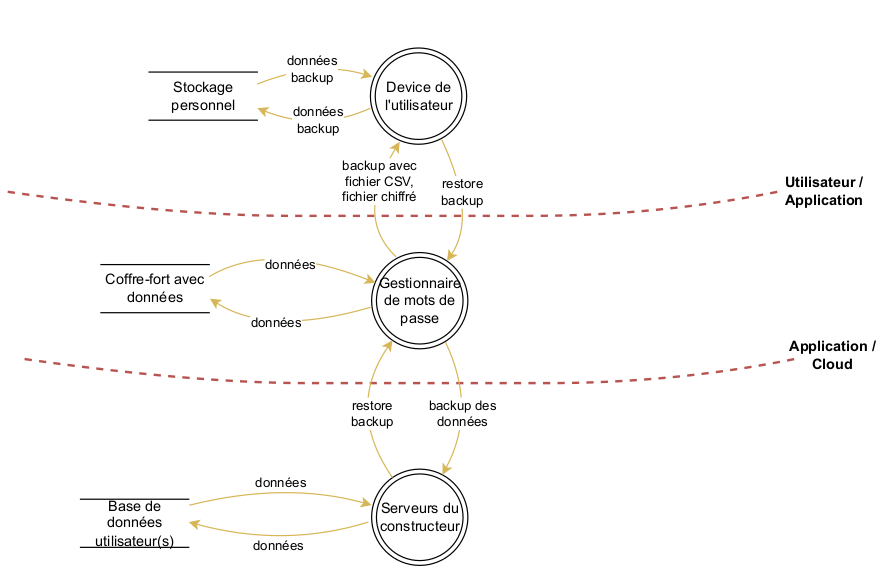
\includegraphics[width=14.5cm]{images/dfd_backup.png}
	\centering
	\caption{Data Flow Diagram pour les applications M2}
\end{figure}

\subsubsection{Identification des risques}

Nous allons procéder exactement comme la section précédente, nous allons premièrement identifier les biens, menaces (avec les sources de menaces et les scénarios), les contrôles, les vulnérabilités ainsi que les conséquences sur l'entreprise afin d'établir une étude complète.

\textbf{Identification des biens}

Ci-dessous les biens présents lors du processus de sauvegarde de données dans un gestionnaire de mots de passe local-based ou cloud/local-based.

\begin{table}[H]
	\centering
	\resizebox{\textwidth}{!}{\begin{tabular}{lll}
			\hline
			Code & Bien                                & Description                                                           \\ \hline
			A1   & Serveurs du constructeur                     & Serveurs qui stockent les données des utilisateur dans le cloud               \\
			A2 & Sauvegardes & Fichiers ou emplacements contenant les sauvegardes des données \\
			\hline
	\end{tabular}}
	\caption{Biens des gestionnaires de mots de passe M2}
\end{table}
\textbf{Identification des sources de menaces}

Nous allons identifier toutes les sources de menaces possibles qui pourraient survenir dans le cadre de backups de données d'un gestionnaire de mots de passe. 

\begin{table}[H]
	\centering
	\begin{tabular}{cll}
		\hline
		Code & Source de menace                & Motivations                               \\ \hline
		S1   & Hackers & Amusement, gloire, challenge, argent, ego \\
		S2   & Script kiddies                  & Curiosité, ego, argent, amusement         \\
		S3   & Concurrent                      & Espionnage, réutilisation de contenu      \\
		S4   & Cybercrime                      & Argent, destruction de données            \\
		S5   & Accident humain                 & -                                         \\
		S6   & Problèmes techniques            & -                                         \\ \hline
	\end{tabular}
	\caption{Sources de menaces des gestionnaires de mots de passe M2}
\end{table}

Ci-dessous, se trouve un tableau avec différents scénarios d'attaques. Nous utilisons le modèle STRIDE afin de définir tous les types de menaces. 

\begin{table}[H]
	\centering
	\resizebox{\textwidth}{!}{\begin{tabular}{ccclll}
			\hline
			& Code & Code du bien & Scénario de menace                                                                                                            & Type de menace                & Source de menace  \\ \hline
			1 & T3   & A1           & \begin{tabular}[c]{@{}l@{}}Communication non chiffrée entre gestionnaire\\ de mots de passe et serveurs\end{tabular}                                                                                  & \textit{Information Disclosure}          & S1, S2, S4, S6   \\
			2 & T3   & A1           & MITM (Interception de données non-chiffrées)                                                                                  & \textit{Information Disclosure}          & S1, S2, S4, S6   \\
			3 & T4   & A1           & DoS                                                                                                                           & \textit{Denial of service}           & S1, S2, S4, S6    		\\
			4 & T5   & A1           & Perte des données utilisateurs dû à un serveur down                                                                                                                           & \textit{Equipment failure}           & S5, S6   	\\
			5 & T3   & A2          & Récupération du backup en clair sur le device du client                                                                                  & \textit{Information Disclosure}          & S1, S2, S3, S4, S6   \\	
			6 & T3   & A2          & Sauvegarde corrompue                                                                                 & \textit{Information Disclosure}          & S5, S6   \\	
			7 & T3   & A2          & Perte de la sauvegarde sur device utilisateur                                                                                 & \textit{Information Disclosure}          & S1, S2, S3, S4, S6   \\	
						8 & T3   & A2           & Vols de backups non protégés sur le serveur                                                                                  & \textit{Information disclosure} & S1, S2, S4, S6         \\
						
			\\\\	\hline 
			\multicolumn{6}{l}{A1 = Serveurs du constructeur | A2 = Sauvegardes}\\ \hline
	\end{tabular}}
	\caption{Scénarios et types d'attaques possibles sur M2}
\end{table}

\textbf{Identification des contrôles}

Dans cette partie, nous nous concentrons uniquement sur la fonctionnalité de backup, ainsi, la liste des contrôles existants n'est pas grande. 

L'unique contrôle que l'on peut citer, qui est fait de manière indirect, est que la sauvegarde sur les serveurs du constructeur est entièrement chiffrée. Étant donné que dans leurs bases de données utilisateurs, le coffre-fort est toujours chiffré grâce au \textit{Zero-knowledge}, naturellement le backup le sera aussi. Cela nous garantit que les données ne sont pas connues des serveurs et sont protégées de quelconques attaques sur ces derniers.

Au niveau du device utilisateur, il est possible d'effectuer des contrôles mais c'est à l'utilisateur de s'assurer que les données sont stockées dans un emplacement sécurisé et à l'abri de toute manipulation malveillante.

\textbf{Identification des vulnérabilités}

Pour chaque actif identifié au préalable, nous allons analyser les vulnérabilités qui pourraient être présentes. Nous allons également ajouter la sévérité de la vulnérabilité. 

\begin{table}[H]
	\centering
	\resizebox{\textwidth}{!}{\begin{tabular}{cll}
			\hline
			Bien                   & Vulnérabilité                                                                                                          & Sévérité de la vulnérabilité   \\ \hline
			A1                     & Backup non effectué sur les serveurs                                                                                            & Critique                        \\
			A1                     & Communication non chiffrée                                                                                                  & Critique                     \\
			A1                     & Infrastructure des serveurs pas assez stable                                                                      & Haut                         \\
			A1                     & \begin{tabular}[c]{@{}l@{}}Infrastructure des serveurs du constructeur pas \\   protégée à quelconques intrusions physiques \end{tabular}                                                                      & Bas                         \\
			A2                    & Manque de chiffrement dans les sauvegardes sur serveurs ou device utilisateur                                                                                            & Critique                        \\
			A2                    & Sauvegarde stockée dans un répertoire personnel non protégé                                                                                    & Moyen                        \\
			A2                     &  Sauvegarde CSV stockée dans un emplacement non sécurisé                                                                                 & Moyen                       \\			
			\\ \\ \hline
			\multicolumn{3}{l}{A1 = Serveurs du constructeur | A2 = Sauvegardes}\\ \hline
	\end{tabular}}
	\caption{Vulnérabilités présentes dans les gestionnaires de mots de passe M2}
\end{table}

\textbf{Identifications des conséquences}

Pour chaque bien défini plus haut, nous allons ajouter les conséquences qu'il pourrait y avoir dans le cas d'attaques, ainsi que ce que nous souhaitons garantir.

\begin{table}[H]
	\centering
	\resizebox{\textwidth}{!}{	\begin{tabular}{lll}
			\hline
			Bien                     & Conséquences     & Garanties                                                                                             \\ \hline
			Serveurs du constructeur (A1)         & Perte de réputation et d'image, pertes de données      & Disponibilité, intégrité, confidentialité                                                                           \\
			Sauvegardes (A2)     & Perte de réputation et d'image, perte de données        & Confidentialité, intégrité des données             \\ \hline
	\end{tabular}}
	\caption{Conséquences des menaces sur l'entreprise}
\end{table}

\subsubsection{Analyse des risques}
Ainsi, dans cette partie, nous allons analyser l'impact des conséquences ainsi que la probabilité que chaque scénario d'attaque identifié puisse se produire. Pour cela, nous allons utiliser plusieurs notations différentes; pour les conséquences nous aurons les niveaux suivants:

\begin{table}[H]
	\centering
	\resizebox{\textwidth}{!}{\begin{tabular}{cclllll}
			\hline 
			Bien & Menace & Scénario                                                                                                                     & Impact des conséquences & Probabilité  & Niveau de risque \\ \hline
			A1   & T3           & \begin{tabular}[c]{@{}l@{}}Communication non chiffrée entre gestionnaire\\ de mots de passe et serveurs\end{tabular}                                                                          &    Catastrophique            & Peu probable      &      Moyen       \\
			A1   & T3           & MITM (Interception de données non-chiffrées) &      Catastrophique          &   Peu probable  &     Moyen        \\
			A1   & T4         & DoS              &       Modéré         & Possible      & Moyen              \\
			A1   & T5        & Perte des données utilisateurs dû à un serveur down                                                                                       &        Catastrophique           &         Peu probable &          Moyen   \\
			A2  & T3         & Récupération du backup en clair sur le device du client                                                                                                    &     Modéré              &   Probable   &      Moyen       \\
			A2   & T3         & Sauvegarde corrompue                                                                                    &         Modéré          &   Rare   &      Bas       \\
			
			A2   & T3          & Perte de la sauvegarde sur device utilisateur            &        Mineur           &  Possible    & Moyen               \\
			A2   & T3           & Vols de backups non protégés sur le serveur     &   Catastrophique        &  Peu probable &   Moyen          \\
			\\\\ \hline 
			\multicolumn{6}{l}{A1 = Serveurs du constructeur | A2 = Sauvegardes }\\ 
			\multicolumn{6}{l}{T1 = Spoofing | T2 = Elevation of privileges | T3 = Information Disclosure | T4 = Denial of service | T5 = Equipment failure | T6 = Tampering}\\ 
			\hline
	\end{tabular}}
	\caption{Analyse des risques de chaque scénario de menace sur M2}
\end{table}
\newpage
\subsection{M3 Synchronisation}

Cette section effectue une analyse de menaces sur la fonctionnalité de synchronisation des gestionnaires de mots de passe. Elle permet de synchroniser les données d'un utilisateur sur un ou plusieurs de ses devices. Cette option concerne uniquement les gestionnaires de mots de passe qui fonctionnent avec le cloud. Ainsi, l'application communique en continu avec les serveurs du constructeur. De plus, nous allons effectuer une analyse sur les fonctionnalités qu'un gestionnaire cloud-based peut proposer, par exemple l'auto-complétion des champs de formulaires.

Nous avons créé un DFD afin de comprendre comment les communications fonctionnent:

\begin{figure}[H]
	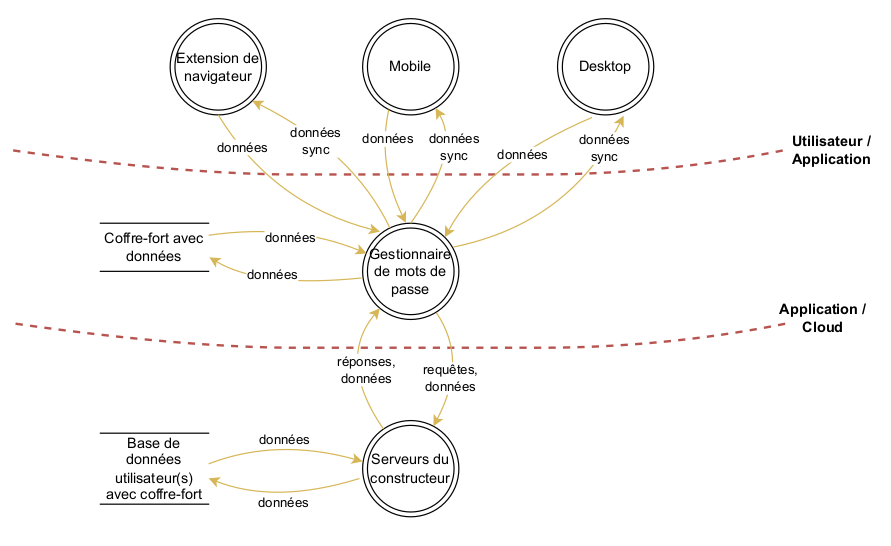
\includegraphics[width=13cm]{images/dfd_sync.png}
	\centering
	\caption{Data Flow Diagram pour les synchronisations}
\end{figure}

\subsubsection{Identification des risques}

Nous allons procéder exactement comme la section précédente, nous allons premièrement identifier les biens, menaces (avec les sources de menaces et les scénarios), les contrôles, les vulnérabilités ainsi que les conséquences sur l'entreprise afin d'établir une étude complète.

\textbf{Identification des biens}

Ci-dessous les biens présents lors du processus de sauvegarde de données dans un gestionnaire de mots de passe cloud-based.

\begin{table}[H]
	\centering
	\resizebox{\textwidth}{!}{\begin{tabular}{lll}
			\hline
			Code & Bien                                & Description                                                           \\ \hline
		A1   & Gestionnaire de mots de passe & L'application du gestionnaire de mots de passe                      \\
A2   & Coffre-fort                     & Base de données avec toutes les informations stockées                \\
			A3 & Serveurs du constructeur & Serveurs qui stockent les données des utilisateur dans le cloud \\
			\hline
	\end{tabular}}
	\caption{Biens des gestionnaires de mots de passe M3}
\end{table}
\textbf{Identification des sources de menaces}

Nous allons identifier toutes les sources de menaces possibles qui pourraient survenir dans le cadre de synchronisations de données d'un gestionnaire de mots de passe. 

\begin{table}[H]
	\centering
	\begin{tabular}{cll}
		\hline
		Code & Source de menace                & Motivations                               \\ \hline
		S1   & Hackers & Amusement, gloire, challenge, argent, ego \\
		S2   & Script kiddies                  & Curiosité, ego, argent, amusement         \\
		S3   & Concurrent                      & Espionnage, réutilisation de contenu      \\
		S4   & Cybercrime                      & Argent, destruction de données            \\
		S5   & Accident humain                 & -                                         \\
		S6   & Problèmes techniques            & -                                         \\ \hline
	\end{tabular}
	\caption{Sources de menaces des gestionnaires de mots de passe M3}
\end{table}

Ci-dessous, se trouve un tableau avec différents scénarios d'attaques. Nous utilisons le modèle STRIDE afin de définir tous les types de menaces. 

\begin{table}[H]
	\centering
	\resizebox{\textwidth}{!}{\begin{tabular}{ccclll}
			\hline
			& Code & Code du bien & Scénario de menace                                                                                                            & Type de menace                & Source de menace  \\ \hline
			1 & T1   & A1           & Phishing en imitant une page de connexion                                                                                     & \textit{Spoofing}   & S1, S2, S3, S4     \\
			2 & T1   & A1           & \begin{tabular}[c]{@{}l@{}}Attaque XSS avec les champs de connexion\\ auto-complétés\end{tabular}                             & \textit{Spoofing}     & S1, S2, S4          \\	
			3 & T3   & A1           & Clickjacking                                                                                                                            & \textit{Information Disclosure}           & S1, S2, S4  \\
			4 & T3   & A3           & \begin{tabular}[c]{@{}l@{}}Communication non chiffrée entre gestionnaire\\ de mots de passe et serveurs\end{tabular}                                                                                  & \textit{Information Disclosure}          & S1, S2, S4, S6   \\
			5 & T3   & A3, A2           & MITM (Interception de données non-chiffrées)                                                                                  & \textit{Information Disclosure}          & S1, S2, S4, S6   \\
			6 & T4   & A3           & DoS                                                                                                                           & \textit{Denial of service}           & S1, S2, S4, S6    		\\
			7 & T5   & A3           & Perte des données utilisateurs dû à un serveur down                                                                                                                           & \textit{Equipment failure}           & S5, S6   	\\
	
			8 & T3  & A3           & Vols de données non protégées sur le serveur                                                                                  & \textit{Information disclosure} & S1, S2, S4, S6          \\				
			\\\\	\hline 
			\multicolumn{6}{l}{A1 = Gestionnaire de mots de passe | A2 = Coffre-fort | A3 = Serveurs du constructeur}\\ \hline
	\end{tabular}}
	\caption{Scénarios et types d'attaques possibles sur M3}
\end{table}

\textbf{Identification des contrôles}

Il est possible de citer quelques contrôles concernant la fonctionnalité de synchronisation de données. 

Premièrement, pour la communication avec le serveurs, tous les gestionnaires de mots de passe cloud-based utilisent le protocole HTTPS afin garantir une communication chiffrée. 

Les données synchronisée sur le device de l'utilisateur sont chiffrées et peuvent être déchiffrées dès le moment où l'utilisateur a entré le bon master password lors de sa connexion au gestionnaire de mots de passe.

Finalement, pour l'auto-complétion des champs de connexion, certains s'assurent que l'utilisateur valide s'il veut vraiment remplir ce champ afin d'éviter d'entrer les données sensibles dans des pages web clonées malveillantes.

\textbf{Identification des vulnérabilités}

Pour chaque actif identifié au préalable, nous allons analyser les vulnérabilités qui pourraient être présentes. Nous allons également ajouter la sévérité de la vulnérabilité. 

\begin{table}[H]
	\centering\resizebox{\textwidth}{!}{\begin{tabular}{cll}
			\hline
			Bien                   & Vulnérabilité                                                                                                          & Sévérité de la vulnérabilité   \\ \hline
			A1 & Auto-complétion de champs sans une interaction avec l'utilisateur          & Moyen             \\
			A1                     & Utilisation de critères de correspondance faibles lors de l'auto-complétion & Moyen           \\
			A1 & Règles d'auto-complétion HTTP ne différencie pas HTTP et HTTPS                                                                                                           & Haut           \\		
							A2                & Utilisation d'algorithmes de chiffrement plus recommandés ou trop faibles   & Haut      \\	
										A3                     & Communication non chiffrée                                                                                                  & Critique                     \\	
			A3                     & Infrastructure des serveurs pas assez stable                                                                      & Haut                         \\
			A3                     & \begin{tabular}[c]{@{}l@{}}Infrastructure des serveurs du constructeur pas protégée à quelconques intrusions \\ physiques\end{tabular}                                                                     & Bas                         \\		
			\\ \\ \hline
			\multicolumn{3}{l}{A1 = Gestionnaire de mots de passe | A2 = Coffre-fort | A3 = Serveurs du constructeur}\\ \hline
	\end{tabular}}
	\caption{Vulnérabilités présentes dans les gestionnaires de mots de passe M3}
\end{table}

\textbf{Identifications des conséquences}

Pour chaque bien défini plus haut, nous allons ajouter les conséquences qu'il pourrait y avoir dans le cas d'attaques, ainsi que ce que nous souhaitons garantir.

\begin{table}[H]
	\centering
	\resizebox{\textwidth}{!}{	\begin{tabular}{lll}
			\hline
			Bien                     & Conséquences     & Garanties                                                                                             \\ \hline
					Application (A1)         & Perte de réputation et d'image      & Disponibilité, intégrité                                                                           \\
			Base de données (A2)     & Perte de réputation et d'image, perte de données        & Confidentialité, intégrité des données             \\
			Serveurs du constructeur (A3)     & Perte de réputation et d'image, perte de données        & Disponibilité, confidentialité, intégrité des données             \\\hline
	\end{tabular}}
	\caption{Conséquences des menaces sur l'entreprise}
\end{table}

\subsubsection{Analyse des risques}
Ainsi, dans cette partie, nous allons analyser l'impact des conséquences ainsi que la probabilité que chaque scénario d'attaque identifié puisse se produire. Pour cela, nous allons utiliser plusieurs notations différentes; pour les conséquences nous aurons les niveaux suivants:


\begin{table}[H]
	\centering
	\resizebox{\textwidth}{!}{\begin{tabular}{cclllll}
			\hline 
			Bien & Menace & Scénario                                                                                                                     & Impact des conséquences & Probabilité  & Niveau de risque \\ \hline
			A1   & T1           & Phishing en imitant une page de connexion                                                                                         &    Modéré            &   Possible    &     Moyen        \\
			A1   & T1           & \begin{tabular}[c]{@{}l@{}}Attaque XSS avec les champs de connexion\\ auto-complétés\end{tabular}  &    Important            &    Possible  &   Moyen          \\
			A1   & T3           & Clickjacking  &     Modéré           &  Possible    &    Moyen         \\
			A3   & T3         & \begin{tabular}[c]{@{}l@{}}Communication non chiffrée entre gestionnaire\\ de mots de passe et serveurs\end{tabular}                    &       Catastrophique         &  Peu probable    &   Moyen           \\
			A3, A2  & T3       & MITM (Interception de données non-chiffrées)                                                                                      &      Catastrophique             &    Peu probable      &      Moyen       \\
			A3  & T4         & DoS                                                                                                   &      Modéré             &   Possible   &    Moyen         \\
			A3   & T5         & Perte des données utilisateurs dû à un serveur down                                                                                   &        Catastrophique           &     Peu probable &    Moyen         \\
			
			A3   & T3          & Vols de données non protégées sur le serveur           &   Important                &  Rare    &          Moyen     \\
			\\\\ \hline 
			\multicolumn{6}{l}{A1 = Gestionnaire de mots de passe | A2 = Coffre-fort | A3 = Serveurs du constructeur }\\ 
			\multicolumn{6}{l}{T1 = Spoofing | T2 = Elevation of privileges | T3 = Information Disclosure | T4 = Denial of service | T5 = Equipment failure | T6 = Tampering}\\ 
			\hline
	\end{tabular}}
	\caption{Analyse des risques de chaque scénario de menaces sur M3}
\end{table}
\newpage
\subsection{M4 Partage}

Nous consacrons cette section à la fonctionnalité de partage de données qui est présente sur les gestionnaires de mots de passe cloud/local-based. Afin de mieux comprendre le processus, nous avons effectué un DFD qui explique comment un objet d'un utilisateur est partagé vers un autre utilisateur:

\begin{figure}[H]
	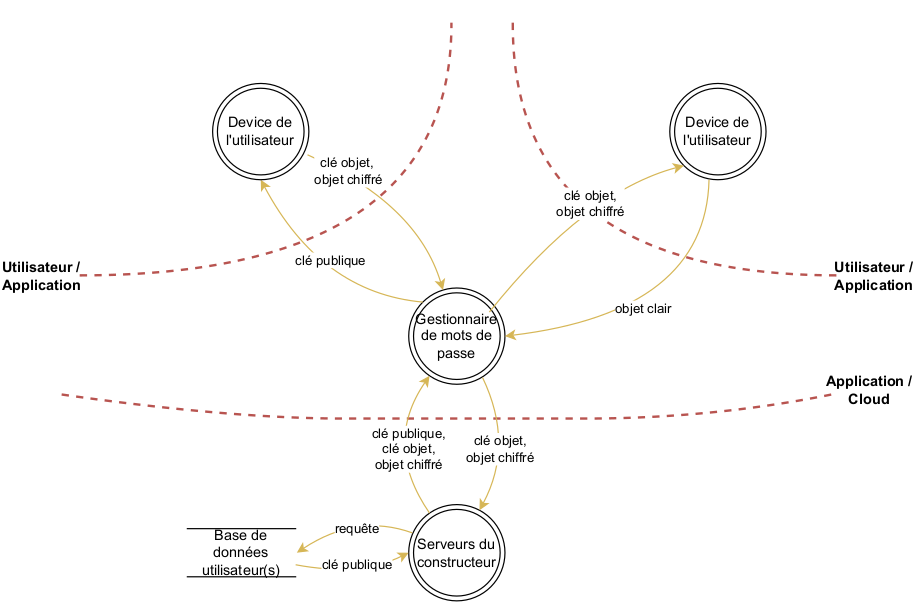
\includegraphics[width=14.5cm]{images/dfd_share.png}
	\centering
	\caption{Data Flow Diagram pour les partages de données}
\end{figure}

\subsubsection{Identification des risques}

Nous allons procéder exactement comme la section précédente, nous allons premièrement identifier les biens, menaces (avec les sources de menaces et les scénarios), les contrôles, les vulnérabilités ainsi que les conséquences sur l'entreprise afin d'établir une étude complète.

\textbf{Identification des biens}

Ci-dessous les biens présents lors du processus de partage entre deux utilisateurs.

\begin{table}[H]
	\centering
	\resizebox{\textwidth}{!}{\begin{tabular}{lll}
			\hline
			Code & Bien                                & Description                                                           \\ \hline
			A1   & Serveurs du constructeur                     & Serveurs qui stockent les données des utilisateur dans le cloud               \\
			A2 & Données partagées & Données qui sont partagées entre utilisateurs \\
			\hline
	\end{tabular}}
	\caption{Biens des gestionnaires de mots de passe M4}
\end{table}

\textbf{Identification des sources de menaces}

Nous allons identifier toutes les sources de menaces possibles qui pourraient survenir dans le cadre de partage de données d'un gestionnaire de mots de passe. 

\begin{table}[H]
	\centering
	\begin{tabular}{cll}
		\hline
		Code & Source de menace                & Motivations                               \\ \hline
		S1   & Hackers & Amusement, gloire, challenge, argent, ego \\
		S2   & Script kiddies                  & Curiosité, ego, argent, amusement         \\
		S3   & Concurrent                      & Espionnage, réutilisation de contenu      \\
		S4   & Cybercrime                      & Argent, destruction de données            \\
		S5   & Accident humain                 & -                                         \\
		S6   & Problèmes techniques            & -                                         \\ \hline
	\end{tabular}
	\caption{Sources de menaces des gestionnaires de mots de passe M4}
\end{table}

Ci-dessous, se trouve un tableau avec différents scénarios d'attaques. Nous utilisons le modèle STRIDE afin de définir tous les types de menaces. 
\begin{table}[H]
	\centering
	\resizebox{\textwidth}{!}{\begin{tabular}{ccclll}
			\hline
			& Code & Code du bien & Scénario de menace                                                                                                            & Type de menace                & Source de menace  \\ \hline
			1 & T3   & A1           & \begin{tabular}[c]{@{}l@{}}Communication non chiffrée entre gestionnaire\\ de mots de passe et serveurs\end{tabular}                                                                                  & \textit{Information Disclosure}          & S1, S2, S4, S6   \\
			2 & T3   & A1           & MITM (Interception de données non-chiffrées)                                                                                  & \textit{Information Disclosure}          & S1, S2, S4, S6   \\
			3 & T1 & A1 & Utilisateur auquel on partage des données n'est pas le bon & \textit{Spoofing} & S1, S2, S4, S6 \\
			4 & T3 & A2 & Donnée partagée non-chiffrée sur les serveurs du constructeur & \textit{Information Disclosure} & S1, S2, S4, S6 \\
			\\\\	\hline 
			\multicolumn{6}{l}{A1 = Serveurs du constructeur | A2 = Données partagées}\\ \hline
	\end{tabular}}
	\caption{Scénarios et types d'attaques possibles sur M4}
\end{table}

\textbf{Identification des contrôles}

Au niveau des contrôles effectuées lors du partage de données entre utilisateurs, il en existe quelques-uns.

Nous n'allons pas citer les contrôles que nous avons déjà pu expliquer dans les autres parties à propos de la communication des serveurs et de l'architecture \textit{Zero-knowledge}, néanmoins nous pouvons ajouter qu'ils s'assurent que même les données à partager sont chiffrées sur les serveurs et que la clé pour chiffrer l'objet est bien chiffrée avec la clé publique de l'utilisateur.

Les serveurs du constructeur contrôlent également que l'utilisateur a qui on demande sa clé publique est vraiment le bon afin d'éviter que des attaquants se fassent passer pour quelqu'un d'autre. Sur certains gestionnaires de mots de passe, ils s'assurent que la clé corresponde à l'e-mail adresse de l'utilisateur (cependant l'identité de la personne n'est pas contrôlée). 

\textbf{Identification des vulnérabilités}

Pour chaque actif identifié au préalable, nous allons analyser les vulnérabilités qui pourraient être présentes. Nous allons également ajouter la sévérité de la vulnérabilité. 

\begin{table}[H]
	\centering
	\resizebox{\textwidth}{!}{\begin{tabular}{cll}
			\hline
			Bien                   & Vulnérabilité                                                                                                          & Sévérité de la vulnérabilité   \\ \hline
			A1                     & Communication non chiffrée                                                                                                  & Critique                     \\
			A1                     & Manque de chiffrement lorsque les données sont envoyées sur les serveurs	& Critique \\
			A1 & Manque de contrôle au niveau de l'identité de la personne & Moyen \\
			A2 & Non chiffrement de données	sensibles & Critique \\
			\\ \\ \hline
			\multicolumn{3}{l}{A1 = Serveurs du constructeur | A2 = Données partagées}\\ \hline
	\end{tabular}}
	\caption{Vulnérabilités présentes dans les gestionnaires de mots de passe M4}
\end{table}

\textbf{Identifications des conséquences}

Pour chaque bien défini plus haut, nous allons ajouter les conséquences qu'il pourrait y avoir dans le cas d'attaques, ainsi que ce que nous souhaitons garantir.

\begin{table}[H]
	\centering
	\resizebox{\textwidth}{!}{	\begin{tabular}{lll}
			\hline
			Bien                     & Conséquences     & Garanties                                                                                             \\ \hline
			Serveurs du constructeur (A1)         & Perte de réputation et d'image, pertes de données      & Disponibilité, intégrité, confidentialité                                                                           \\
			Données partagées (A2)     & Perte de réputation et d'image, perte de données        & Confidentialité, intégrité des données             \\ \hline
	\end{tabular}}
	\caption{Conséquences des menaces sur l'entreprise}
\end{table}

\subsubsection{Analyse des risques}
Ainsi, dans cette partie, nous allons analyser l'impact des conséquences ainsi que la probabilité que chaque scénario d'attaque identifié puisse se produire. Pour cela, nous allons utiliser plusieurs notations différentes; pour les conséquences nous aurons les niveaux suivants:

\begin{table}[H]
	\centering
	\resizebox{\textwidth}{!}{\begin{tabular}{cclllll}
			\hline 
			Bien & Menace & Scénario                                                                                                                     & Impact des conséquences & Probabilité  & Niveau de risque \\ \hline
			A1   & T3           & \begin{tabular}[c]{@{}l@{}}Communication non chiffrée entre gestionnaire\\ de mots de passe et serveurs\end{tabular}                                                                          &     Catastrophique           &  Peu probable     &     Moyen        \\
			A1   & T3           & MITM (Interception de données non-chiffrées) &   Catastrophique            &  Peu probable    &       Moyen      \\
			A1   & T1        & Utilisateur auquel on partage des données n'est pas le bon              &       Important            &  Probable   &     Haut         \\
			A2   & T3        & Donnée partagée non-chiffrée sur les serveurs du constructeur                                                                                      &       Important            &    Peu probable      &       Moyen      \\
			\\\\ \hline 
			\multicolumn{6}{l}{A1 = Serveurs du constructeur | A2 = Données partagées }\\ 
			\multicolumn{6}{l}{T1 = Spoofing | T2 = Elevation of privileges | T3 = Information Disclosure | T4 = Denial of service | T5 = Equipment failure | T6 = Tampering}\\ 
			\hline
	\end{tabular}}
	\caption{Analyse des risques de chaque scénario de menaces sur M4}
\end{table}

\newpage

\subsection{M5 Application bas-niveau}

La dernière partie de cette analyse de menaces concerne la sécurité des gestionnaires de mots de passe et de tous ses composants, donc tout le bas-niveau. Cela inclut le stockage des données sensibles (clés, coffre-fort, master password) en mémoire RAM ainsi que sur le disque (fichiers de sauvegardes). Puis, nous aborderons les processus de chiffrement et génération des clés.

Ci-dessous un schéma représentant l'architecture bas-niveau des applications.

\begin{figure}[H]
	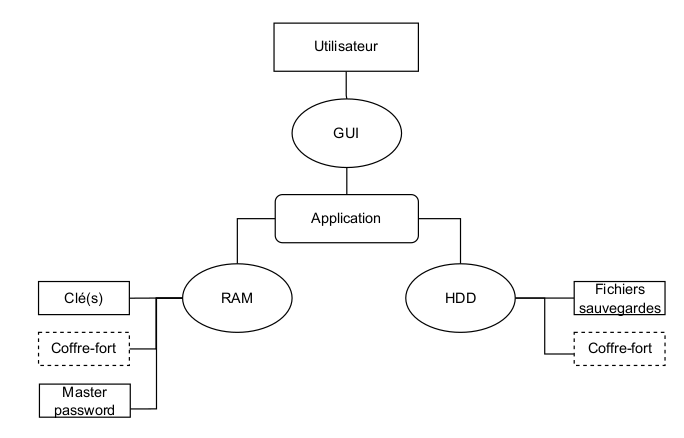
\includegraphics[width=14.5cm]{images/dfd_low.png}
	\centering
	\caption{Schéma bas-niveau des gestionnaires de mots de passe}
\end{figure}

\subsubsection{Identification des risques}

Nous allons procéder exactement comme la section précédente, nous allons premièrement identifier les biens, menaces (avec les sources de menaces et les scénarios), les contrôles, les vulnérabilités ainsi que les conséquences sur l'entreprise afin d'établir une étude complète.

\textbf{Identification des biens}

Ci-dessous les biens concernant la sécurité bas-niveau des gestionnaires de mots de passe.

\begin{table}[H]
	\centering
	\resizebox{\textwidth}{!}{\begin{tabular}{lll}
			\hline
			Code & Bien                                & Description                                                 \\ \hline
			A1   & Coffre-fort                    &   Base de données avec toutes les informations stockées             \\
			A2 & Master password & Mot de passe principal afin de déchiffrer le coffre-fort \\
			A3 & Clés & Clé(s) de chiffrement et privée(s) de l'utilisateur  \\			
			\hline
	\end{tabular}}
	\caption{Biens des gestionnaires de mots de passe M5}
\end{table}
\textbf{Identification des sources de menaces}

Nous allons identifier toutes les sources de menaces possibles qui pourraient survenir au niveau bas-niveau de l'application. 

\begin{table}[H]
	\centering
	\begin{tabular}{cll}
		\hline
		Code & Source de menace                & Motivations                               \\ \hline
		S1   & Hackers & Amusement, gloire, challenge, argent, ego \\
		S2   & Script kiddies                  & Curiosité, ego, argent, amusement         \\
		S3   & Concurrent                      & Espionnage, réutilisation de contenu      \\
		S4   & Cybercrime                      & Argent, destruction de données            \\
		S5   & Accident humain                 & -                                         \\
		S6   & Problèmes techniques            & -                                         \\ \hline
	\end{tabular}
	\caption{Sources de menaces des gestionnaires de mots de passe M5}
\end{table}

Ci-dessous, se trouve un tableau avec différents scénarios d'attaques. Nous utilisons le modèle STRIDE afin de définir tous les types de menaces. 
\begin{table}[H]
	\centering
	\resizebox{\textwidth}{!}{\begin{tabular}{ccclll}
			\hline
			& Code & Code du bien & Scénario de menace                                                                                                            & Type de menace                & Source de menace  \\ \hline
			1 & T3   & A1           & Récupération de données sensibles en clair sur le disque                                                                      & \textit{Information disclosure}      & S1, S2, S4 \\
			2 & T3   & A1           & \begin{tabular}[c]{@{}l@{}}Récupération du coffre-fort et déchiffrement\\ dû à un algorithme trop simple\end{tabular}  & \textit{Information disclosure}    & S1, S2, S4    \\
			3 & T3   & A1, A2, A3           & Récupération de données sensibles en mémoire                                                                                  & \textit{Information Disclosure}    & S1, S2, S4     \\
			4 & T3   & A3           & Récupération de la clé de chiffrement en mémoire                                                                              & \textit{Information Disclosure}    & S1, S2, S4 \\
			5 & T3   & A3           & Brute-force de clé                                                                                                            & \textit{Information Disclosure}    & S1, S2, S4    \\                                                     
			
			\\\\	\hline 
			\multicolumn{6}{l}{A1 = Coffre-fort | A2 = Master password | A3 = Clés}\\ \hline
	\end{tabular}}
	\caption{Scénarios et types d'attaques possibles sur M5}
\end{table}

\textbf{Identification des contrôles}

Le contrôle qui est présent sur toutes les applications est que chaque utilisateur possède une clé de chiffrement différente, qui est dérivée avec son master password. Même si ce dernier est le même, la clé ne sera pas pareille dû au salt qui est soit aléatoire soit le username, qui est unique. Les algorithmes choisis sont forts (voir \ref{crypto}) et sont recommandés pour la dérivation des clés. Ainsi, la clé est protégée contre le brute-force ou les attaques par dictionnaire. Néanmoins, il est quand même important d'avoir un master password fort\footnote{Ce qu'on considère un mot de passe fort; au moins une majuscule, une minuscule, un chiffre et 11 caractères}, ce qui n'est pas demandé dans tous les gestionnaires de mots de passe lors de l'inscription de l'utilisateur.

Pour le chiffrement des données, les gestionnaires de mots de passe utilisent AES-256. L'algorithme est également encore recommandé en 2022.

Au niveau de la protection mémoire, certains proposent une protection des données sensibles dans le processus (avec DPAPI ou Chacha20) et les données sont effacées sur le disque dès que le processus s'arrête. En se basant sur une étude\cite{iseexploit}, la mémoire est en général bien protégée lorsque le gestionnaire dans l'état \textit{Not Running}, cependant dès le moment où le gestionnaire est dans l'état \textit{Unlock} ou \textit{Locked}, les secrets et le master password sont plus exposés. 

\textbf{Identification des vulnérabilités}

Pour chaque actif identifié au préalable, nous allons analyser les vulnérabilités qui pourraient être présentes. Nous allons également ajouter la sévérité de la vulnérabilité. 

\begin{table}[H]
	\centering
	\resizebox{\textwidth}{!}{\begin{tabular}{cll}
			\hline
			Bien                   & Vulnérabilité                                                                                                          & Sévérité de la vulnérabilité   \\ \hline
				A1                 & \begin{tabular}[c]{@{}l@{}}Utilisation d'algorithmes de chiffrement plus recommandés ou \\ trop faibles\end{tabular}   & Haut                       \\
				A1, A2, A3                     & Aucune protection de la mémoire du processus                                                                           & Haut         \\
				A1, A2, A3                     & Option \textit{remember me}                                                                                                   & Haut                \\
				\multicolumn{1}{c}{A1, A2, A3} & Données non nettoyées de la mémoire lors de l'arrêt du processus           & Haut                   \\	

A3                     & Dérivation des clés trop simple                                                                                        & Moyen             \\											
			\\ \\ \hline
			\multicolumn{3}{l}{A1 = Coffre-fort | A2 = Master password | A3 = Clés}\\ \hline
	\end{tabular}}
	\caption{Vulnérabilités présentes dans les gestionnaires de mots de passe M5}
\end{table}

\textbf{Identifications des conséquences}

Pour chaque bien défini plus haut, nous allons ajouter les conséquences qu'il pourrait y avoir dans le cas d'attaques, ainsi que ce que nous souhaitons garantir.

\begin{table}[H]
	\centering
	\resizebox{\textwidth}{!}{	\begin{tabular}{lll}
			\hline
			Bien                     & Conséquences     & Garanties                                                                                             \\ \hline
			Coffre-fort (A1)         & Perte de réputation et d'image, pertes de données      & Intégrité, confidentialité                                                                           \\
			Master password (A2)     & Perte de réputation et d'image, perte de données        & Confidentialité, intégrité des données             \\
			Clés (A3)     & Perte de réputation et d'image, perte de données        & Confidentialité, intégrité              \\ \hline
	\end{tabular}}
	\caption{Conséquences des menaces sur l'entreprise}
\end{table}

\subsubsection{Analyse des risques}
Ainsi, dans cette partie, nous allons analyser l'impact des conséquences ainsi que la probabilité que chaque scénario d'attaque identifié puisse se produire. Pour cela, nous allons utiliser plusieurs notations différentes; pour les conséquences nous aurons les niveaux suivants:

\begin{table}[H]
	\centering
	\resizebox{\textwidth}{!}{\begin{tabular}{cclllll}
			\hline 
			Bien & Menace & Scénario                                                                                                                     & Impact des conséquences & Probabilité  & Niveau de risque \\ \hline
			A1   & T3           & Récupération des données sensibles en clair sur le disque &     Important           &   Probable   &   Haut          \\
			A1   & T3         & \begin{tabular}[c]{@{}l@{}}Récupération du coffre-fort et déchiffrement\\ dû à un algorithme trop simple\end{tabular}             &    Important            &   Peu probable   &     Moyen         \\
			A1, A2, A3   & T3        & Récupération de données sensibles en mémoire                                                                            &     Important              &     Probable     &   Haut          \\
			A3  & T3         & Récupération de la clé de chiffrement en mémoire                                                                           &    Important               &   Probable   &       Haut      \\
			A3   & T3         & Brute-force de clé                                                                                  &     Important              &  Rare    &    Moyen         \\
			
			\\\\ \hline 
			\multicolumn{6}{l}{A1 = Coffre-fort | A2 = Master password | A3 = Clés}\\ 
			\multicolumn{6}{l}{T1 = Spoofing | T2 = Elevation of privileges | T3 = Information Disclosure | T4 = Denial of service | T5 = Equipment failure | T6 = Tampering}\\ 
			\hline
	\end{tabular}}
	\caption{Analyse des risques de chaque scénario de menace sur M5}
\end{table}

\subsection{Évaluation des risques}

Cette étape sert à évaluer si les risques sont acceptables ou s'ils ont besoin d'un traitement supplémentaires, c'est-à-dire une mitigation. Nous avons défini à l'étape précédente le niveau de risque de chaque scénario de menace. En résumé, nous avons:

\begin{itemize}
	\item Bas: 2
	\item Moyen: 17
	\item Haut: 6
\end{itemize} 

Ainsi, nous pouvons définir que les tous les scénarios de menaces ayant un niveau de risque bas peuvent être acceptés par l'entreprise, néanmoins ces derniers ne doivent pas être oubliés et mis de côté. Pour les niveaux de risques moyen et haut, il est nécessaire d'appliquer une mitigation et de surveiller les menaces. 

\subsection{Traitement des risques}
Dans cette section, nous allons définir les contre-mesures à entreprendre afin d'éviter au maximum les menaces que nous avons identifié plus haut. Comme précisé dans le paragraphe de l'identification des contrôles, beaucoup de choses sont déjà mises en place par les constructeurs et sont efficaces contre les attaques. Néanmoins, nous pouvons ajouter quelques contre-mesures qui ne sont pas ou peu effectuées par les quelques candidats que nous avons sélectionnés au préalable. Ainsi, nous allons sélectionner les risques qui ont été qualifiés comme moyen ou haut et nous allons proposer des contre-mesures possibles.

	\begin{table}[H]
	\centering
	\resizebox{\textwidth}{!}{\begin{tabular}{l|l}
		\hline
		\textbf{Menace}                                    & \textbf{Contre-mesures }                                                                                                                                                                                                                                                                                                          \\ \hline
		Master password faible                    & \begin{tabular}[c]{@{}l@{}}- Ajouter des contrôles lors de l'inscription de l'utilisateur en lui demandant un mot de passe fort\\ - Proposer un master password fort généré aléatoirement par l'application\end{tabular}                                                                                                 \\ \hline
		Temps de session trop long                & - Ajouter un temps d'expiration de session et verrouiller le gestionnaire après ce temps                                                                                                                                                                                                                                 \\ \hline
		Presse-papier non nettoyé                 & - Après un temps court, nettoyer le presse-papier de l'utilisateur                                                                                                                                                                                                                                                       \\ \hline
		Brute-force               & 
		\begin{tabular}[c]{@{}l@{}} - Ajouter un nombre d'essais maximum \\ - Ajouter une politique de master password forte\end{tabular}                                                                               \\ \hline
		Phishing en clonant une page de connexion & \begin{tabular}[c]{@{}l@{}}- Appliquer un meilleur critère de match lors de l'auto-complétion des champs\\ de connexion\\ - Demander à l'utilisateur de valider l'auto-complétion         \\ - Sensibilisation auprès des utilisateurs  \end{tabular}                                                                                                                \\ \hline
		Clickjacking                              & - Bloquer l'utilisation de Javascript à l'aide d'API sécurisées                                                                                                                                                                                                                                                          \\ \hline
		Communication non-chiffrée                & \begin{tabular}[c]{@{}l@{}}- Ajouter HTTPS pour la communication avec le serveur\\ - Éviter d'envoyer le master password ou des clés de chiffrement ou\\ privée au serveur\\ - Chiffrer toutes les données avant de les envoyer dans le cloud\end{tabular}                                                               \\ \hline
		Dérivation des clés trop simple           & \begin{tabular}[c]{@{}l@{}}- Utiliser un algorithme recommandé et fort (PBKDF2-SHA2 par exemple)\\ - Une clé de chiffrement unique par utilisateur pour éviter le brute force\end{tabular}                                                                                                                               \\ \hline
		Perte de données                          & \begin{tabular}[c]{@{}l@{}}- Si cloud-based / browser-based, effectuer des backups sur les serveurs chaque\\ nuit\\ - Mettre à disposition la fonctionnalité de backup pour les particuliers pour les \\ faire en local\\ - Exportation des données CSV et les stocker dans un endroit chiffrer et sécurisé\end{tabular} \\ \hline
		Manque de protection dans la mémoire      & \begin{tabular}[c]{@{}l@{}}- Nettoyage de mémoire lorsque le gestionnaire est dans l'état locked\\ - Protection des données sensible avec des APIs pour limiter l'exposition\\ de secrets\end{tabular}                                                                                                                   \\ \hline
		\multicolumn{1}{l|}{Option remember me}  & \multicolumn{1}{l}{- Désactivation de mode offline avec les gestionnaires cloud-based et browser-based}                                                                                                                                                                                                                 \\ \hline
		Manque de protection du disque & - Utiliser un chiffrement du disque entier \\ \hline
	\end{tabular}}
\caption{Contre-mesures possibles pour les gestionnaires}
\end{table}

\section{Exigences sécuritaires à respecter} 
Dans cette dernière section de l'analyse de menaces, nous allons établir une liste d'exigences sécuritaires que les gestionnaires de mots de passe doivent respecter afin de se définir sécurisé et afin de protéger les données sensibles au maximum. Nous allons premièrement identifier toutes les exigences générales puis nous allons les définir plus en détails afin d'expliquer ce que nous souhaitons garantir.
%\multirow{5}{*}{\STAB{\rotatebox[origin=c]{90}{\textbf{Chiffrement}}}}
Pour les identifier, nous allons nous référencer à notre analyse de menaces puis nous allons également nous baser sur le standard de OWASP \textit{Application Security Verification Standard}\cite{ASVS}. 
\begin{landscape}
	\centering
	\fontsize{8}{11}\selectfont
\begin{longtable}[H]{c|l|l}
			\hline
			\multicolumn{1}{c|}{\textbf{Type}} & \multicolumn{1}{c|}{\textbf{Description de l'exigence}} & \multicolumn{1}{c}{\textbf{Commentaire}}  \\ \hline
			\multirow{5}{*}{\textbf{Chiffrement}}      & \begin{tabular}[c]{@{}l@{}}Le coffre-fort de l'utilisateur doit impérativement être chiffré avec\\ un algorithme ainsi qu'une taille de clé qui sont recommandés\end{tabular}         & \begin{tabular}[c]{@{}l@{}}Nous pouvons nous baser sur les recommandations \\ du report de ECRYPT\cite{ecrypt}. Au mieux, l'algorithme \\ devrait être encore recommandé pour une utilisation \\  future.\end{tabular} \\ \cline{2-3} 
			& \begin{tabular}[c]{@{}l@{}}Le chiffrement doit être end-to-end pour assurer la protection de\\ données lors du transport dans le cloud\end{tabular}                                   & \begin{tabular}[c]{@{}l@{}}Concerne les gestionnaires qui fonctionnent avec le\\ cloud et font de la synchronisations de données\end{tabular}                                                                                       \\ \cline{2-3} 
			& Le chiffrement doit être fait côté client, donc en local                                                                                                                              & \begin{tabular}[c]{@{}l@{}}Afin d'éviter que des données claires soient stockés sur\\ les serveurs\end{tabular}                                                                                                                     \\ \cline{2-3} 
			& L'architecture Zero-knowledge doit être respectée                                                                                                                                     & Cette exigence est identique à la précédente                                                                                                                                                                                        \\ \cline{2-3} 
			& \begin{tabular}[c]{@{}l@{}}La communication entre l'utilisateur et les serveurs doit être \\ chiffrée avec un algorithme recommandé\end{tabular}                                      & HTTPS est la meilleure solution de chiffrement                                                                                                                                                                                      \\ \hline
			\multirow{5}{*}{\textbf{Clés de chiffrement}} & \begin{tabular}[c]{@{}l@{}}La dérivation de clé.s doit se baser sur des algorithmes \\ Password-Based Key Derivation et doit être recommandé\end{tabular}                             & \begin{tabular}[c]{@{}l@{}}Les plus courants sont Argon2 et PBKDF2 (associé à \\ une fonction de hash)\end{tabular}                                                                                                                 \\ \cline{2-3} 
			& Le salt doit être unique                                                                                                                                                              & \begin{tabular}[c]{@{}l@{}}Si on utilise le username ou l'adresse e-mail, il faut\\ absolument s'assurer que ce dernier soit unique lors de\\ l'inscription de l'utilisateur\end{tabular}                                           \\ \cline{2-3} 
			& Le salt doit être aléatoire (si on n'utilise pas le username)                                                                                                                         & \begin{tabular}[c]{@{}l@{}}Utiliser un pseudo-nombre généré aléatoirement \\ pour s'assurer qu'il soit correctement aléatoire\end{tabular}                                                                                          \\ \cline{2-3} 
			& \begin{tabular}[c]{@{}l@{}}Les clés et la salt doivent être stockés localement dans la mémoire\\ du processus\end{tabular}                                                            &                                                                                                                                                                                                                                     \\ \cline{2-3} 
			& \begin{tabular}[c]{@{}l@{}}Les clés de chiffrement ne doivent jamais être envoyées \\ aux serveurs et rester en local\end{tabular}                                                    & Pour les gestionnaires qui utilisent le cloud                                                                                                                                                                                       \\ \hline
			\multirow{3}{*}{\textbf{Authentification}}   & \begin{tabular}[c]{@{}l@{}}Authentifier les données avec un schéma sûr, comme Encrypt-\\ then-MAC\end{tabular}                                                                        & \begin{tabular}[c]{@{}l@{}}Nécessaire pour les gestionnaires qui ne \\ fonctionnent qu'en local\end{tabular}                                                                                                                        \\ \cline{2-3} 
			& Authentifier les utilisateurs auprès des serveurs du constrtucteur                                                                                                                    & \begin{tabular}[c]{@{}l@{}}Pour les gestionnaires qui fonctionnent \\ également avec le cloud\end{tabular}                                                                                                                          \\ \cline{2-3} 
			& \begin{tabular}[c]{@{}l@{}}Hash d'authentification stocké dans la base de données des \\ serveurs doit être chiffré\end{tabular}                                                      & \begin{tabular}[c]{@{}l@{}}Hash utilisé pour le comparer avec celui que le client\\ envoie afin d'approuver l'authentification\end{tabular}                                                                                         \\ \hline
			\multirow{5}{*}{\textbf{Master password}}     & \begin{tabular}[c]{@{}l@{}}Le master password doit respecter des critères lors de\\ l'inscription de l'utilisateur\end{tabular}                                                       & \begin{tabular}[c]{@{}l@{}}Pour que le master password soit fort et qu'on évite au\\ maximum des attaques sur mots de passe\end{tabular}                                                                                            \\ \cline{2-3} 
			& Le master password ne devrait jamais être stocké en mémoire                                                                                                                           & \begin{tabular}[c]{@{}l@{}}À moins que des précautions de protection de mémoire \\ aient été prises et qu'on ne puisse pas le voir en clair\end{tabular}                                                                            \\ \cline{2-3} 
			& La fonctionnalité Remember me est fortement déconseillée                                                                                                                              & \begin{tabular}[c]{@{}l@{}}Dû au fait que le master password puisse être stocké en\\ mémoire\end{tabular}                                                                                                                           \\ \cline{2-3} 
			& \begin{tabular}[c]{@{}l@{}}Demander obligatoirement le 2FA ou MFA à l'utilisateur lors de\\ son inscription\end{tabular}                                                              & Cela permet d'ajouter une couche sécuritaire                                                                                                                                                                                        \\ \cline{2-3} 
			& \begin{tabular}[c]{@{}l@{}}Le master password devrait rester localement et ne devrait jamais\\ être transmis aux serveurs\end{tabular}                                                & Pour les gestionnaires qui fonctionnent avec le cloud                                                                                                                                                                               \\ \hline
			\textbf{Session}                              & Un temps de session doit être ajouté obligatoirement                                                                                                                                  & \begin{tabular}[c]{@{}l@{}}Le gestionnaire se place dans un état Locked après\\ ce temps\end{tabular}                                                                                                                               \\ \hline
			\multirow{4}{*}{\textbf{Mémoire}}             & \begin{tabular}[c]{@{}l@{}}Dans l'état Not Running, aucune donnée qui puisse faire\\ compromettre la base de données sur le disque ne doit être \\ stockée sur le disque\end{tabular} & \begin{tabular}[c]{@{}l@{}}Par exemple, le master password ou une clé\\ de chiffrement dans un fichier de configuration\end{tabular}                                                                                                \\ \cline{2-3} 
			& \begin{tabular}[c]{@{}l@{}}Dans l'état Unlocked, il devrait pas être possible d'extraire le\\ master password de la mémoire\end{tabular}                                              &                                                                                                                                                                                                                                     \\ \cline{2-3} 
			& \begin{tabular}[c]{@{}l@{}}Dans l'état Unlocked, il ne devrait pas être possible d'extraire de\\ la mémoire des éléments déchiffrés avec lesquels on n'a pas interagi\end{tabular}    & \begin{tabular}[c]{@{}l@{}}Une interaction peut être afficher, copier ou encore\\ l'accès aux mots de passe\end{tabular}                                                                                                            \\ \cline{2-3} 
			& \begin{tabular}[c]{@{}l@{}}Dans l'état Locked, il ne devrait pas être possible d'extraire\\ n'importe quelle donnée sensible\end{tabular}                                             & \begin{tabular}[c]{@{}l@{}}Toutes les données doivent être effacées de la \\ mémoire\end{tabular}                                                                                                                                   \\ \hline
			\multirow{4}{*}{\textbf{Partage de données}}  & \begin{tabular}[c]{@{}l@{}}Les clés privées ne devraient être accessibles qu'aux utilisateurs\\ concernés\end{tabular}                                                                &                                                                                                                                                                                                                                     \\ \cline{2-3} 
			& \begin{tabular}[c]{@{}l@{}}Les clés privées doivent rester en local et ne jamais être envoyé\\ aux serveurs\end{tabular}                                                              &                                                                                                                                                                                                                                     \\ \cline{2-3} 
			& Les clés publiques et les identités liées doivent être vérifiées                                                                                                                      & \begin{tabular}[c]{@{}l@{}}Afin de s'assurer que l'utilisateur a qui on demande\\ sa clé est le bon\end{tabular}                                                                                                                    \\ \cline{2-3} 
			& \begin{tabular}[c]{@{}l@{}}L'élément a partager et sa clé de chiffrement doivent être chiffrés\\ localement\end{tabular}                                                              &                                                                                                                                                                                                                                     \\ \hline
			\textbf{Backup}                               & Les sauvegardes stockées sur les serveurs doivent être chiffrées                                                                                                                      &                                                                                                                                                                                                                                     \\ \hline
			\textbf{Presse-papier}                        & \begin{tabular}[c]{@{}l@{}}Le presse-papier doit être nettoyé après un court instant (10-40s),\\ l'historique du presse-papier doit également être nettoyé\end{tabular}               & Pour éviter le sniffing de presse-papier                                                                                                                                                                                            \\ \hline
			\multirow{5}{*}{\textbf{Attaques web-based}   }                & \begin{tabular}[c]{@{}l@{}}Pour l'auto-complétion des champs, il est nécessaire de demander\\ l'autorisation à l'utilisateur pour remplir le champs\end{tabular}                      & Cela peut faire évitter des attaques de phishing                                                                                                                                                                                    \\ \cline{2-3} 
			& \begin{tabular}[c]{@{}l@{}}Les critères de matching pour les URLs lors de l'auto-complétion\\ doivent être stricts\end{tabular}                                                       &                                                                                                                                                                                                                                     \\ \cline{2-3} 
			& Éviter d'ignorer les sous-domaines de l'URL                                                                                                                                           & \begin{tabular}[c]{@{}l@{}}Afin de s'assurer qu'il n'est pas possible de voler les\\ identifiants du domaine parent\end{tabular}                                                                                                    \\ \cline{2-3} 
			& \begin{tabular}[c]{@{}l@{}}Il faudrait faire la différence entre HTTP et HTTPS lors du remplissage\\ automatique des champs\end{tabular}                                              & \begin{tabular}[c]{@{}l@{}}Pour éviter une attaque MITM et de remplir une page\\ clônée HTTP d'un  site initalement HTTPS\end{tabular}                                                                                              \\ \cline{2-3} 
			& Il faut bloquer l'exécution Javascript   \\\hline
						\caption{Exigences sécuritaires}  
                                                                                                                                         
\end{longtable}

\end{landscape}